% 08_distillazione.tex — Capitolo 8: Knowledge distillation: il teacher insegna al MLP.
% Documento didattico "Intelligenza artificiale nel progetto supervised_telemedicina".

\chapter{Knowledge distillation: il teacher insegna al MLP}\label{cap:distillazione}

Nei capitoli precedenti abbiamo incontrato i due protagonisti del progetto: il
teacher rule-based (capitolo~\ref{cap:teacher}), che assegna la classe di
rischio con soglie nette e leggibili, e l'MLP (capitolo~\ref{cap:reti}), che
approssima funzioni non lineari con confini morbidi. In questo capitolo li
mettiamo insieme: il teacher \emph{etichetta} il dataset sintetico e il
MLP \emph{impara da quelle etichette}. Questa tecnica si chiama
\textbf{knowledge distillation}, ed è il cuore di \progetto{}.

\section{L'idea generale}\label{sec:idea-generale}

La \emph{knowledge distillation} (distillazione della conoscenza) è
l'idea di trasferire la conoscenza di un modello in un altro: un modello
\emph{teacher} (l'insegnante) produce le risposte, e un modello
\emph{student} (lo studente) impara a riprodurle. L'articolo di Hinton,
Vinyals e Dean \cite{hinton2015distilling} ha reso celebre questa
impostazione: lo studente non impara dai dati grezzi, ma dalle risposte del
teacher, che fungono da ``appunti già pronti''.

Un'analogia da programmazione: un insegnante esperto non consegna allo
studente il libro di testo da leggere da zero, ma prepara degli appunti che
distillano i concetti essenziali. Lo studente che studia quegli appunti non
rilegge mai il libro originale, eppure ne eredita la conoscenza. Nel nostro
caso il ``libro di testo'' sono le regole cliniche scritte a mano, e gli
``appunti'' sono le etichette che il teacher assegna a ogni campione del
dataset.

La distillazione ha un vantaggio teorico importante: il teacher può essere
qualsiasi cosa — un sistema a regole, un ensemble di modelli, una rete
enorme — mentre lo studente può essere un modello piccolo, veloce e
leggero. Il progetto \progetto{} porta questa idea all'estremo: il teacher
è un insieme di \codice{if}/\codice{elif} su soglie cliniche, e lo studente
è un MLP con 323 parametri (capitolo~\ref{cap:reti}).

\section{Perché distillare un sistema a regole in una rete}\label{sec:perche-distillare}

Perché sostituire un sistema a regole, semplice e trasparente, con una rete
neurale? Le ragioni sono quattro.

\begin{itemize}
  \item \textbf{Velocità di inferenza}: le regole richiedono una cascata di
        confronti condizionali, un'istruzione alla volta; l'MLP invece è un
        prodotto di matrici, calcolabile in un colpo solo con numpy. Con un
        batch di pazienti, la rete esegue l'inferenza in un'unica operazione
        vettoriale.
  \item \textbf{Robustezza ai confini}: le soglie del teacher sono
        \emph{gradini}: basta un decimo di grado per cambiare classe. La
        rete produce confini \emph{sfumati}: il passaggio da
        \classe{basso} a \classe{alto} è graduale, quindi un piccolo rumore
        di misura non fa cambiare bruscamente la risposta.
  \item \textbf{Confidenza}: il teacher risponde solo con la classe; l'MLP
        produce una distribuzione di probabilità (softmax). Sapere
        \emph{quanto} è sicuro il sistema è prezioso in clinica, come
        vedremo nel capitolo~\ref{cap:sicurezza}.
  \item \textbf{Manutenibilità}: le regole vanno aggiornate a mano, rischio
        di errori e incoerenze compreso (capitolo~\ref{cap:teacher}). Il
        MLP, invece, si \emph{riaddestra}: se il teacher cambia, basta
        rigenerare le etichette e riaddestrare la rete.
\end{itemize}

C'è anche un motivo strategico: un modello addestrato può in futuro
imparare anche da dati reali, mentre un sistema a regole no. La
distillazione è il ponte che ci porta dal mondo delle regole al mondo
dell'apprendimento.

\section{La pipeline del progetto}\label{sec:pipeline-progetto}

La figura~\ref{fig:diagramma-distillazione} riassume l'intera pipeline
della distillazione in \progetto{}: il teacher rule-based etichetta i
campioni generati dal generatore sintetico, il dataset etichettato
addestra il MLP, e a runtime il safety gate decide quando fidarsi della
rete.

\begin{figure}[htbp]
  \centering
  % diagramma_distillazione.tex — diagramma TikZ (incluso dai capitoli).
\begin{tikzpicture}[
    nodo/.style={draw, rounded corners=2pt, minimum height=0.9cm, align=center, font=\small},
    freccia/.style={-{Stealth[length=2.5mm]}, thick},
  ]
  \node[nodo, fill=blue!10] (teacher) at (0,0) {Teacher rule-based\\\file{teacher\_rules.py}};
  \node[nodo, fill=green!15] (gen) at (3.4,0) {Generatore sintetico\\\file{synthetic\_generator.py}};
  \node[nodo, fill=orange!15] (ds) at (6.8,0) {Dataset etichettato\\70\,000 campioni};
  \node[nodo, fill=green!15] (mlp) at (10.2,0) {MLP numpy\\6 $\to$ $n$ $\to$ 3};
  \node[nodo, fill=red!15] (gate) at (13.6,0) {Safety gate\\a runtime};
  \draw[freccia] (teacher) -- (gen);
  \draw[freccia] (gen) -- (ds);
  \draw[freccia] (ds) -- (mlp);
  \draw[freccia] (mlp) -- (gate);
  \node[below=0.3cm of ds, font=\scriptsize, align=center] {etichette = decisioni\\del teacher (distillazione)};
\end{tikzpicture}

  \caption{La pipeline della distillazione in \progetto{}: il teacher
  rule-based etichetta i campioni del generatore sintetico; il dataset
  risultante (70\,000 campioni) addestra il MLP; a runtime il safety gate
  decide la risposta finale.}
  \label{fig:diagramma-distillazione}
\end{figure}

Come avviene, nel codice, l'attacco delle etichette ai campioni? Il
generatore sintetico (\file{training/synthetic\_generator.py}) genera un
campione da un profilo clinico, verifica che non cada nella buffer zone
(capitolo~\ref{cap:dati}), poi chiede al teacher la sua classe:

\begin{lstlisting}[caption={Come il teacher etichetta ogni campione in \file{synthetic\_generator.py} (ciclo di \codice{genera\_batch}).}]
nome_profilo = random.choices(_NOMI_PROFILI, weights=_PESI, k=1)[0]
campione = _campiona_profilo(rng, nome_profilo)
if buffer_zone and _in_buffer_zone(campione):
    scartati += 1
    continue
classe = label(campione)          # il teacher assegna la label
if classe == "errore":
    scartati += 1                 # gli input invalidi non finiscono nel dataset
    continue
X[i] = [campione[nome] for nome in FEATURE_ORDER]
y[i] = classe                     # la label del teacher viene attaccata al campione
i += 1
\end{lstlisting}

Il teacher stesso (\file{training/teacher\_rules.py}) è volutamente
minimale: la classe \codice{TeacherRules} non possiede soglie proprie, ma
riusa la funzione \codice{classifica\_rischio} del modulo di sicurezza
(fonte unica delle soglie, capitolo~\ref{cap:teacher}):

\begin{lstlisting}[caption={Il teacher \codice{TeacherRules} in \file{teacher\_rules.py}: nessuna soglia propria, solo riuso della fonte unica.}]
class TeacherRules:
    def label(self, parametri: Any) -> str:
        """Label di rischio: 'basso' | 'medio' | 'alto' | 'errore'."""
        return classifica_rischio(parametri)

    # Alias esplicito per uso in generazione dataset.
    etichetta = label
\end{lstlisting}

Il risultato è un dataset di 70\,000 campioni etichettati — 40\,000 di
train, 10\,000 di validazione, 20\,000 di test (capitolo~\ref{cap:dati}) —
che il training usa per far imparare al MLP la funzione del teacher
(capitolo~\ref{cap:training}).

\section{Regioni di decisione a confronto}\label{sec:regioni-decisione}

Una domanda naturale è: \emph{il MLP ha davvero imparato il teacher?} La
figura~\ref{fig:heatmap-regioni} risponde visivamente: mostra le regioni di
decisione del teacher (a sinistra) e del MLP (a destra), proiettate sul
piano di due feature, con i dati del progetto reale.

\begin{figure}[htbp]
  \centering
  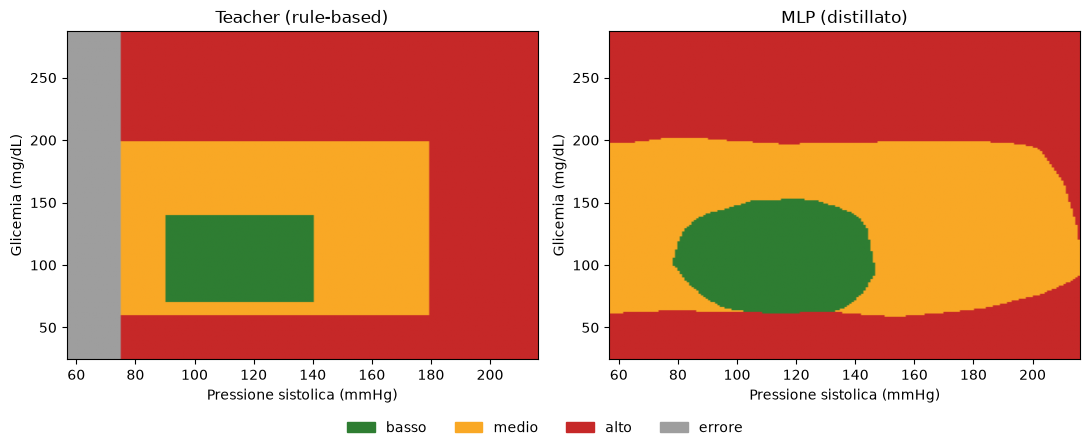
\includegraphics[width=0.85\textwidth]{figure/generate/heatmap_regioni.png}
  \caption{Regioni di decisione a confronto: il teacher rule-based (a
  sinistra) ha confini netti e rettilinei; il MLP (a destra) imita la
  stessa mappa ma con confini morbidi e curvilinei.}
  \label{fig:heatmap-regioni}
\end{figure}

Le due mappe sono quasi sovrapponibili: il MLP ha \emph{imitato} la
struttura del teacher. Le differenze sono nella forma dei confini: dove il
teacher cambia classe di colpo (un gradino), il MLP interpola in modo
graduale. È esattamente la robustezza ai confini di cui parlavamo: nelle
zone vicine a una soglia, il MLP non ``flip-pa'' bruscamente ma produce
probabilità intermedie, segnalando con la confidenza la propria
incertezza.

Questa figura è generata dai dati reali del progetto dal tool
\file{tools/genera\_dashboard.py} e riusata identica dalla dashboard
(capitolo~\ref{cap:riproducibilita}).

\section{I numeri}\label{sec:numeri-distillazione}

Le metriche di valutazione (capitolo~\ref{cap:valutazione}) confermano
l'impressione visiva. Sul test congelato di 20\,000 campioni:

\begin{itemize}
  \item \textbf{accuracy del MLP}: $0.9851$ ($\frac{19702}{20000}$);
  \item \textbf{baseline rule-based}: il teacher applicato alle proprie
        label ha accordo $1.0$ su $20000$ campioni (è l'upper bound per
        costruzione);
  \item \textbf{kappa di Cohen}: $0.9775$;
  \item \textbf{recall del \classe{alto}}: $0.9958$.
\end{itemize}

Il confronto con la baseline è illuminante: l'MLP raggiunge il $98.51\%$
della perfezione del teacher. Il divario di $1.49$ punti percentuali è
fatto di 298 errori sul test congelato. Dove sbaglia la rete? I dati del
report \file{data/models/report.json} lo dicono con precisione: la
distanza media degli errori dalle soglie del teacher è $0.524$ e la
massima $0.681$ — tutti gli errori cadono \emph{vicino ai confini di
decisione}. L'MLP imita il teacher ovunque il gradino è netto e sbaglia
solo dove la classe cambia bruscamente, proprio come previsto dalla teoria
della distillazione.

\begin{esempio}{L'upper bound della distillazione}
L'accordo di $1.0$ del teacher con le proprie label non è una metrica di
qualità clinica: è la misura di \emph{quanto le label del dataset siano
fedeli alle regole}. L'accuracy dell'MLP va letta come ``fedeltà alle
regole sintetiche'', non come accuratezza diagnostica su pazienti reali,
come ricorda l'interpretazione del report \cite{progetto2026}.
\end{esempio}

\section{I limiti della distillazione}\label{sec:limiti-distillazione}

La distillazione è potente, ma ha un limite fondamentale, ben riassunto
dal vecchio adagio dell'informatica: \emph{garbage in, garbage out}.
L'MLP impara dalle etichette del teacher: se il teacher sbaglia, l'MLP
impara l'errore. La qualità dello studente è \emph{limitata dalla qualità
del teacher}, non dai suoi parametri.

Nel nostro progetto questo limite è esplicito: le etichette derivano da
soglie cliniche \emph{arbitrarie} (capitolo~\ref{cap:teacher}), non da un
verdetto di medici su dati reali. L'accuracy di $0.9851$ misura la fedeltà
a quelle soglie, niente di più. La distillazione non crea conoscenza: la
\emph{trasferisce}, e può solo trasferire quella che già c'è.

C'è poi un limite pratico: se le regole cambiano (per esempio perché una
nuova linea guida sposta una soglia), la distillazione va \emph{ripetuta}
— nuovi dati, nuovo training, nuovo report. È il prezzo da pagare per
avere un modello che si aggiorna insieme alle regole, e la base del tema
del prossimo capitolo: come garantire che a runtime il sistema si comporti
in modo sicuro anche quando la rete sbaglia.
